\chapter{Theoretical Background}
This chapter provides the bare minimum theoretical knowledge on electron storage ring physics and particles dynamics needed to state to the reader the optimization problem and the constraints which are involved. A qualitative description of the physics of electron storage rings is presented, followed by a more detailed and more quantitative treatment of single particle dynamics in storage rings.

\section{The physics of electron storage rings}
As mentioned previously, a storage ring is designed to confine bunches of electrons and steer them along a reference closed orbit. The orbit is defined by the bending magnets, the dipoles. The trajectories consist on oscillations about the closed orbit, and focusing of such oscillations toward the closed orbit is provided by gradient fields, mostly coming from quadrupole magnets. Additionally, to correct chromatic aberrations in the beam's motion, i.e. a dependence of focusing with the beam's energy, and guarantee correct focusing despite energy deviations from the nominal value, sextupolar magnetic fields are also introduced, providing fields depending qudratically on the deviations from the nominal orbit. These fields introduce strong nonlinearities in the dynamics.

When having its trajectory bent at the dipoles and insertion devices,
%\footnote{Insertion devices (IDs) consist on arrays of magnetic blocks arranged to provide additional deflection of the beam's trajectory for the production of synchrotron radiation. IDs allow for fine-tuning of the fields and as consequence of the characteristics of the emitted readiation, such as the energy and polarization.}
the beam loses energy in the form of synchrotron radiation. To mantain the beam stored, the energy lost must be replenished. To this aim, radio-frequency (RF) cavities are placed along the ring to provide oscilating electric fields parallel to the longitudinal direction. The work done in the beam by the fields restore its energy.

The radiated photons are emitted in a narrow cone with angular aperture of $1/\gamma$, $\gamma$ being the relativistic Lorentz factor ($\sim 6000$ at SIRIUS storage ring). The photons carry away a fraction of the beam's energy and momentum in both the longitudinal and transverse directions. When passing through RF cavities, only momentum in the longitudinal direction is replenished. The combined effect of radiating photons and passing throgh RF cavities leads to an overall damping of transverse amplitudes.

On the other hand, the quantum nature of the emitted radiation leads to the excitation of transverse oscillations, which is known as quantum excitation. When a photon carries away energy, it depletes the electrons energy by the same amount. It thus changes the reference orbit of the electron in certain regions of the ring (dispersive regions), inducing oscillations. Eventually, equillibrium between radiative damping and quantum excitation is achieved, leading the rms values of each electron's amplitudes to reach a stationary regime.
\todo[inline]{include the case of nondispersive and vertical amplitudes damping}

Each one of the beam's degrees of freedom defines an acceptance: limits which if exceeded can result in instabilities and eventually beam losses. The most obvious acceptance is the transverse acceptance: the beam motion is bounded by a vacuum chamber and colliding with the chamber's physical apperture leads to losses. Additionally, the beam also has an energy acceptance: a tolerance for energy deviations from the nominal value that when exceeded can lead to a suboptimal energetic balance, which, in turn, leads to significant deviations from the nominal orbit and eventually collisions with the vacuum chamber.

The beam is also subject to elastic and inelastic collisions with residual gas molecules within the chamber and also the collisions between electrons within the same bunch, besides other kinds of interactions with wake-fields from other bunches. All these effects can lead to beam-losses and the overall beam loss rate resulting from these combined mechanisms defines the characteristic time scale at which a given electron current survives in the ring. This is the beam lifetime and determines the rate at which injections into the storage ring are required.

Because of the nonlinearities introduced by the sextupole magnets, the transverse acceptances can be limited not solely by the physical aperture available in the vaccum chamber but rather by the amplitudes above which motion is irregular, unstable and unbounded. As already mentioned before, this limiting amplitude is known as the dynamic aperture (DA), a term that can be used to refer to amplitudes in the transverse space $x,y$ or to the phase space coordinates $x, p_x$ and $y, p_y$.

Despite the complicated physics of a fully-coupled dynamics involving the transverse and the energy oscillations and also the damping and the excitation of amplitudes, collective effects and instabilities, for the purpose of this dissertation, it is sufficient to model the motion of a single electron, negletcting radiation losses (and thus the existence of the RF cavities) and any other collective interactions.

In this picture, the electron travels along the ring at the speed of light and executes transverse oscillations in two orthogonal planes. The dynamics takes place in a 4-dimensional phase space which is the  dynamics of two independent quasi-periodic oscillators. These simplfications are justified for our immediate purposes because:
\begin{itemize}
    \item radiation losses/gains and energy oscillations are only significant over a time scale of a couple of turns. Over this period, tens of transverse oscilations take place
    \item the linear and uncoupled dynamics this modeling renders serves as a building block upon which ellaborate modeling can be carried out, incoporating coupling, nonlinearities and perturbations with perturbation theory
    \item why is it ok to ignore collective effects and instabilities?
\end{itemize}

Next, the single-particle dynamics is presented with the aim of defining quantitavely the dynamic aperture and the characteristics of the dynamics in electron strorage rings. Throghout the modelling, optical functions and parameter for the SIRIUS storage rings are also presented.
\section{Motion of charged particles in magnetic fields}
An electron of charge $e$ and momentum of magnitude $p$ follows a circular orbit of radius $\rho$ when interacting with an uniform and time-independent magnetic field of magnitude $B$ directed perpendicularly to the ortbit plane. In such conditions, the Lorentz force law predicts that the relevant quantities are related by
\begin{equation}
    R(p)\equiv B\rho = \frac{p}{e}.
    \label{eq:rigidity}
\end{equation}

Consider now an electron traveling along a curve parametrized by the arclength $s$ with respect to an arbitrary reference point. The interaction with fields $B_x(x,y,s)$  and $B_y(x,y,s)$, both perpendicular to the electron's motion, results in deflections of the trajectory. The deflection angles are given by
    \begin{equation}
        \begin{aligned}
            \dd{\theta_u} & = \frac{\dd{s}}{\rho_u(s)} = \frac{e}{p}B_v(x,y,s)\dd s = \frac{1}{R(p)}B_v(x,y,s)\dd s, \quad u,v=x, y \quad\text{or}\quad y,x.
        \end{aligned}
        \label{eq:deflec_angles}
    \end{equation}
Where \eqref{eq:rigidity} has been used to replace the $p/e$ ratio by the \textit{magnetic rigity} $R(p)$, which is defined as the product of the uniform field strength needed for a beam with momentum $p$ and charge $e$ to perform circular orbit with radius $\rho$. The rigidity depends solely on the electron's momentum/energy and gives the appropriate normalization to evaluate the instantaneous angular deflections in the electron's trajectory caused by magnetic fields.

\todo[inline]{Add deflection figures}

\section{The coordinate system for storage ring dynamics}
As sketched by Figure~\ref{fig:storage_ring}, electrons in a storage ring perform a prescribed nearly circular trajectory close to a reference orbit. A convenient coordinate frame to decribe the dynamics in storge rings can be constructed by imagining a reference particle traveling along a curve drawn by the tip of a vector $\vb{r}_0$, as Fig.~\ref{fig:frenet-serret} shows. The idea is that this particle samples exactly the reference nominal orbit. The particle travels a distance $s$ along the ring, which can be used to parametrize the motion. The triad of direction vectors consists of a vector $\vu{s}$, tangent to the trajectory, a vector $\vu{x}$ normal to it, pointing in the direction at which $\vu{s}$ changes and a vector $\vu{y}=\vu{x}\cross\vu{s}$, bi-normal to the trajectory. This construction leads to a Frenet-Serret reference frame. The deviations from the nominal orbit can be measured in units of the unit vectors in the normal and bi-normal directions, characterizing the transverse dynamics. One may also be concerned with the distance of a given particle from the reference particle itself along the curce. Such differences may arise due to differences in the energy two particles. Since no radiation loss nor gain will be considered in our modeling, the energy and longitudinal deviations from the reference particle are not dynamical quantities, but rather parameters of the dynamics.

Assuming no curvature in the $y$ plane, i.e. that the accelerator defines a curve whose plane is parallel to the facility flat floor, then the unit vectors defining the frame can be calculated by\cite{lee_accelerator_2004}
\begin{equation}
\vu{s}=\dv{\vb{r}_{0}}{s}, \quad \vu{x}=-\rho\dv{\vu{s}}{s}, \quad \vu{y} =  \vu{x}\times\vu{s}.
\end{equation}
where $\rho(s) = \norm{\dv*{\vu{s}}{s}}^{-1}$ is the local curvature radius\footnote{For a circular trajectory, $\vb{r}_0 = (R\cos(s/R), R\sin(s/R), 0)$, $ 0\leq s \leq L$ (check), in the cartesian laboratory frame. $\vu{s}=(-\sin(s/R), \cos(s/R), 0)$, $\dv*{\vu{s}}{s} = -R^{-1}(\cos(s/R),\sin(s/R), 0 )$ and $\rho(s)=R$, justifying the interpretation as curvature radius.}. The vectors evolve along $s$ as prescribed by the Frenet-Serret equations:
\begin{equation}
\dv{\vu{s}}{s}=-\frac{1}{\rho(s)}\vu{x}, \quad\dv{\vu{x}}{s}=\frac{1}{\rho(s)}\vu{s}, \quad \dv{\vu{y}}{s}=0,
\end{equation}
The frame thus depends solely on the geometry of the specified path. Since the curvature is defined by the dipolar fields $B_0(s)$ in the $y$ direction, then, eq.~\eqref{eq:deflec_angles} leads to
    \begin{equation}
        \frac{1}{\rho(s)} = \frac{B_0(s)}{R_0},
        \label{eq:G}
    \end{equation}
where $R_0$ is the rigidity for the beam at the nominal energy.
\begin{figure}[htb]
    \centering
    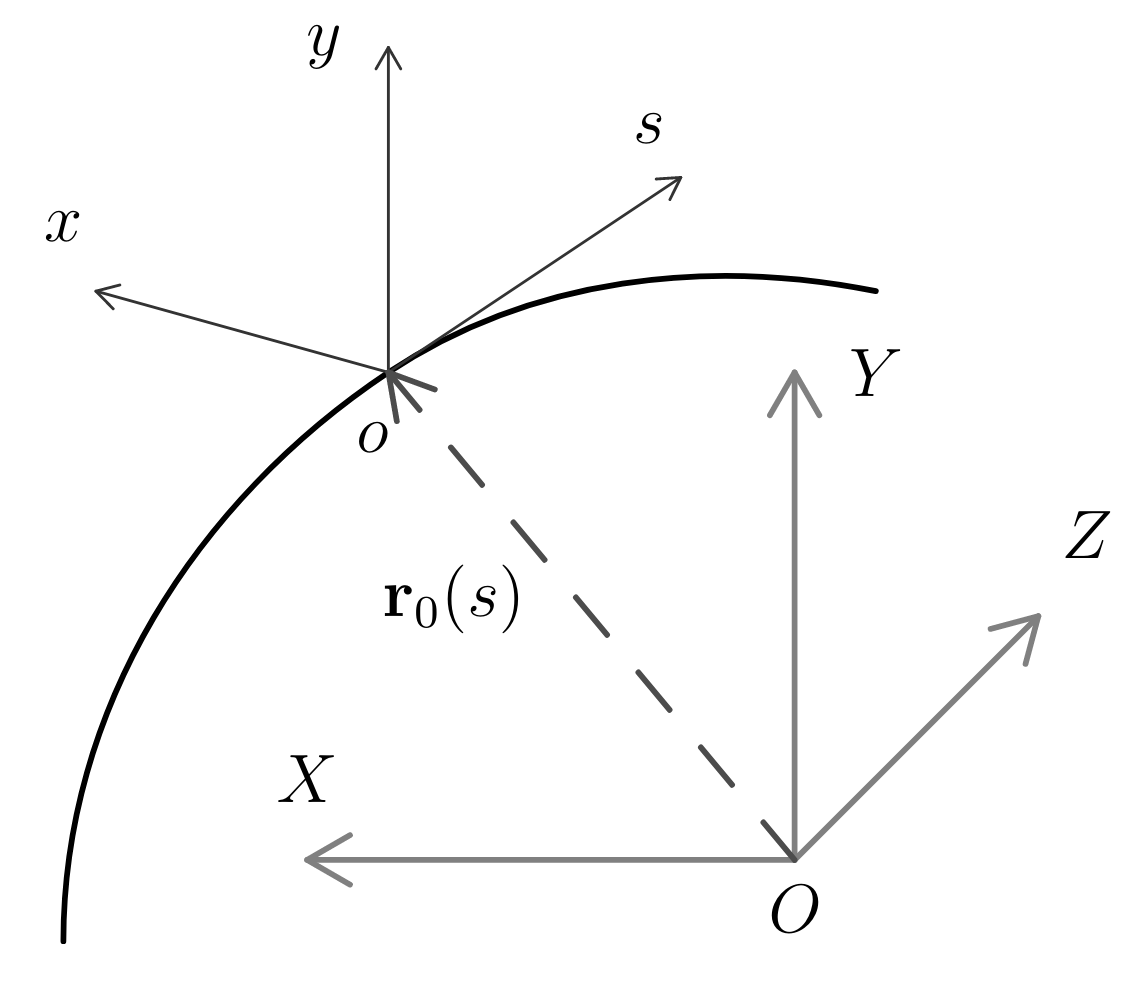
\includegraphics[width=0.6\textwidth]{Images/frenetserret.png}
    \caption{The Frenet-Serret coordinate system. From \cite{huang_beam-based_2019}.}
    \label{fig:frenet-serret}
\end{figure}

\section{Hamiltonian for the relativistic electron}
The dynamics of relativistic electrons influenced by electromagnetic fields $(\Phi, \vb{A})$ is encapsulated by the Hamiltonian \cite{landau_classical_1975}
    \begin{equation*}
        H=\sqrt{m^2c^4+(\vb{P}-q\vb{A})^2c^2}+e\Phi,
    \end{equation*}
 $e$ being the elementary charge and $\vb{P}=\vb{p}+e\vb{A}$ the canonical momentum. The following steps are followed to obtain equations of motion for electrons in the storage ring:
 \begin{itemize}
    \item A canonical transformation to change coordinates is applied in order to describe the motion in terms of the Frenet-Serret frame variables $x$, $y$;
    \item Instead of time $t$, the Hamiltonian and the dynamical variables are described as functions of $s$, the longitudinal position along the ring;
    \item Paraxial approximation: the transverse momenta are assumed to be way smaller than the momentum along the trahectory's tangent direction. This allows the expansion of the the square root in the Hamiltonian as a power series, revealing the expression for an approximate Hamiltonian which can be more easily handled;
    \item Geometric quantities are used: in the paraxial approximation, the canonical momenta for on-energy particles are identified with the derivatives with respect to the parameter $s$ $x^\prime = \dv*{x}{s}$ and $y^\prime = \dv*{y}{s}$, which represent the divergence angles from the nominal orbit;
 \end{itemize}
 All of the transformations and manipulations summarized above can be found in detail in the litereature, such as in Refs.~\cite{lee_accelerator_2004, wiedemann_particle_2015,  wolski_beam_2014}. As mentioned previously, by neglecting RF cavities ($\Phi=0$) and radiation losses, the energy will a constant parameter and the dynamics will consist solely on the transverse degrees of freedom.  In this 4-dimensional dynamics, the set of canonical variables are $(x,p_{x},y , p_{y})$, where the momenta are given by
\begin{equation} p_{x}= x^\prime(1+\delta),\quad p_{y}=y^\prime (1+\delta)\end{equation}
and $\delta$ is the relative deviation from the nominal energy-momentum:
\begin{equation}
    \delta \equiv \frac{P-P_{0}}{P_{0}}\approx\frac{E-E_0}{E_0}.
\end{equation}
The ultra-relativistic approximation $E\approx pc$ was used.

Hamilton's equations for the paraxial-approximated Hamiltonian reveals the equations of motion for the $x$ and $y$ Frenet-Serret coordinates, which read:
\begin{equation}
x^{\prime \prime}=-\frac{(1+G x)^{2}}{1+\delta} \frac{B_{y}}{R_0}+G(1+G x),
\quad
y^{\prime \prime}=\frac{(1+G x)^{2}}{1+\delta} \frac{B_{x}}{R_0},
\label{eq:EOMs}
\end{equation}
where $R_0 = p_0/e$ is the magnetic rigidity of the beam at the nominal energy and $G(s)\equiv\rho^{-1}(s)$ is the inverse local radius of curvature, related to the dipole field as in Eq.~\eqref{eq:G}.
\section{Specification of magnetic fields}
To study the motion, we need to specify the fields $B_x(s)$ and $B_y(s)$ acting on the beam. Since in a storage ring the magnets are arranged as arrays of dipoles, quadrupoles and sextupoles which usually have some symmetry and periodicity, the $B_x(s)$ and $B_y(s)$ functions are generally periodic. If $\ell_{\text{d}}, \ell_{\text{s}}, \ell_{\text{s}}$ are the lengths of dipoles, quadrupoles and sextupoles magnets in a ring, respectively, the magnetic fields are sectionally defined and have the following functional forms
\begin{itemize}
    \item Horizontal Dipole
           \begin{equation} B_x(s) = 0, \quad B_y(s) = B_0, \quad s\in(0,\ell_{\text{d}}),
            \label{eq:dipole}
           \end{equation}
    \item Normal quadrupole
          \begin{equation}B_x = B_1 y, \quad B_y = B_1 x, \quad s\in(0,\ell_{\text{q}}),
            \label{eq:quadrupole}
           \end{equation}
    \item Normal sextupole
          \begin{equation}B_x = B_2xy, \quad B_y = \frac{1}{2}B_2(x^2 - y^2), \quad s\in(0,\ell_{\text{s}}),
            \label{eq:sextupole}
           \end{equation}
\end{itemize}
and zero everywhere else, neglecting the fields of insertion devices. Fields \eqref{eq:dipole}--\eqref{eq:sextupole}  are the so-called \textit{normal multipole fields}. There are also \textit{skew multipole fields}, which couple the horizontal and vertical dynamics. We will neglect skew fields and coupling for now. They can be treated as perturbations in perturbation theory schemes.

In eqs.~\eqref{eq:EOMs}, the magnetic rigidity normalizes all the fields. We therefore define the normalized dipolar, quadrupolar and sextupolar fields as the functions
\begin{equation}
    G(s) = \frac{B_0(s)}{R_0}, \quad K(s) = \frac{B_1(s)}{R_0}, \quad S(s) = \frac{B_2(s)}{R_0}.
    \label{eq:mag_funcs}
\end{equation}
\missingfigure{add plot of the $S$, $K$ and $S$ functions}

\section{Linear Dynamics}
\subsubsection{The linear equations of motion}
Expansion of eqs.~\eqref{eq:EOMs} up to first order in the $x, y, \delta$ variables leads to \cite{sands_physics_1969}
    \begin{equation}
        x^{\prime\prime}+(G^2+K)x=G\delta, \quad
        y^{\prime\prime}-Ky=0.
        \label{eq:linearEOM}
    \end{equation}
    For on-momentum particles, $\delta=0$, both equations are instances of Hill's equations
    \begin{equation}
        u^{\prime\prime}+K_u(s)u = 0,
        \label{eq:Hill}
    \end{equation}
   i.e, a pair of parametric oscillators for $u=x,y$, with $s$-dependent and periodic focusing functions
         $$K_x(s) = G^2(s) + K(s), \quad K_y(s) = - K(s),$$
    the analogues to an oscillator's spring force per unit mass. Motion in the linear approximation thus consists on oscilations around the closed orbit, known as \textit{betatron oscillations}.
\subsubsection{Pseudoharmonic description}
Betatron motion can be cast in a amplitude-phase form. One can show that
\begin{equation}
    u(s) = \sqrt{2\beta_u(s) J_u}\cos(\phi_u(s) + \phi_0),\quad u=x,y,
    \label{eq:pseudo_harmon}
\end{equation}
is a solution to \eqref{eq:Hill} as long as the $\beta_u(s)$ function satifies the boundary-value problem
\begin{equation}
    \frac{1}{2}\beta_{u}^{\prime\prime}+\beta_{u} K_u(s) - \frac{1}{\beta_{u}}\qty(\frac{1}{4}\beta_{u}^{\prime 2} + 1 ) = 0, \quad
        \begin{cases}
            \beta_{u}(0) = \beta_{u}(L)\\ \beta_{u}^{\prime}(0) = \beta_{u}^{\prime}(L)
        \end{cases}
    \label{eq:beta_eq}
\end{equation}
and the phase advance is given by
    \begin{equation}
        \phi_u(s) = \int_{0}^{s}\frac{1}{\beta_u(\sigma)}\dd\sigma.
   \end{equation}
The motion is oscillatory, non-harmonic and non-periodic. The oscillations envelope is the square-root of the beta functions $\beta_u(s)$, which for the SIRIUS storage ring are shown in Fig.~\ref{betafunc}.
\begin{figure}[htb]
    \centering
    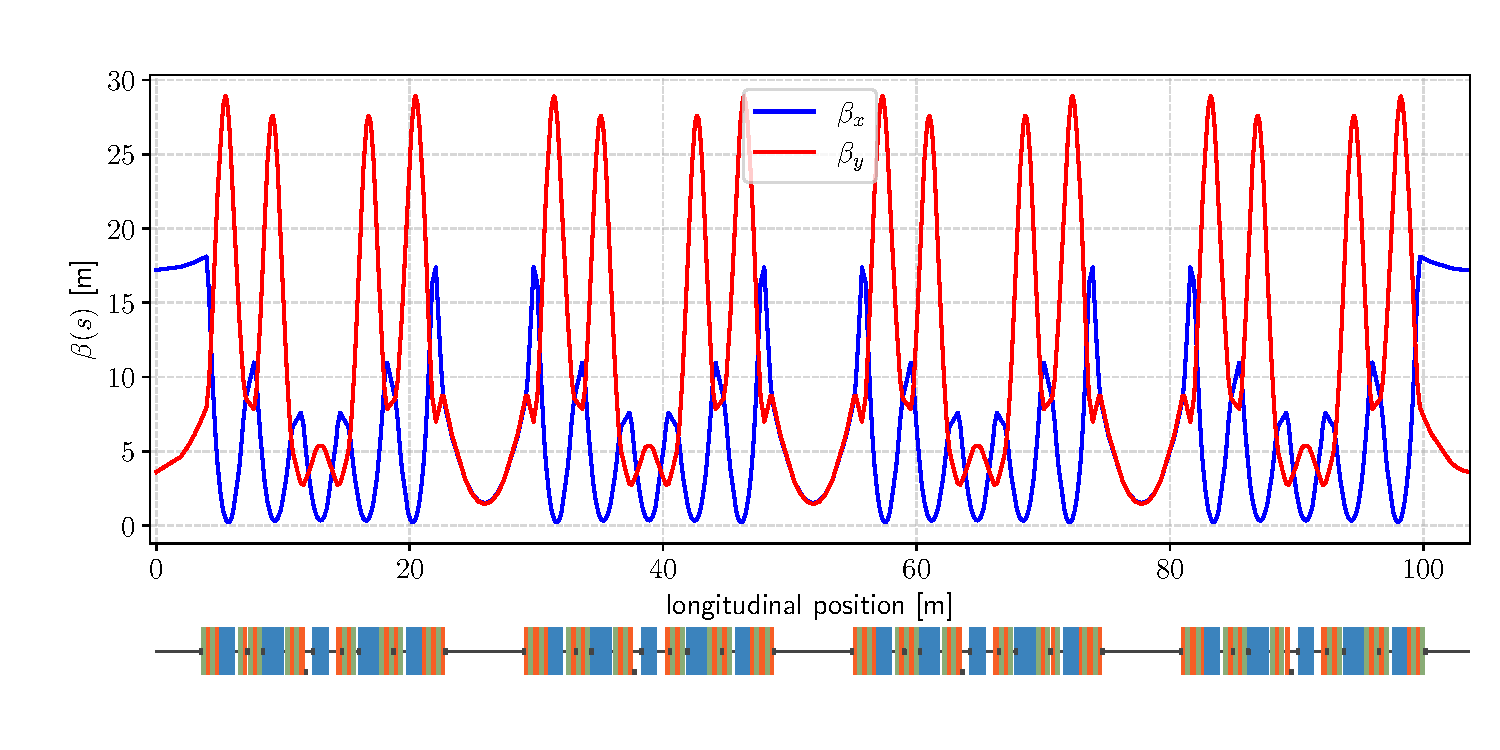
\includegraphics[width=\textwidth]{Images/beta_functions.pdf}
    \caption{Betatron functions for the SIRIUS storage ring. Colored blocks represent the magnets of the accelerator lattice: blue for dipoles, orange for quadrupoles and green for sextupoles. The ring has a 5-fold symmetry, with the lattice and betatron function repeating the same pattern shown above five times up to $s=518~\unit{m}$}
    \label{betafunc}
\end{figure}
\subsubsection{The tune}
An important feature of the dynamics is the \textit{tune}: the phase advance over a revolution along the ring
\begin{equation*}
    \nu_u=\frac{1}{2\pi}\int_{s}^{s+L}\frac{\dd \sigma}{\beta_u(\sigma)}\equiv\frac{1}{2\pi}\oint\frac{\dd s}{\beta_u(s)}.
\end{equation*}
The tune reveals the number of transverse oscilations per revolution. The nominual tunes for SIRIUS storage ring are $(\nu_x, \nu_y)=(49.08, 14.14)$.

When studying the effects of perturbations and nonlinearities acting on the beam, one finds the tunes are a critical variables in determining the beam's response. More specifically, the tunes impact over disturbances amplifiction factors, which are greatest when tunes are close to integer numbers.

\subsubsection{Turn-by-turn motion}
If one keeps track of the time evolution of the the $u, u^\prime$ variables at a fixed position along the ring, plotting them in a phase space, one realizes the the quasi-periodic motion traces out ellipses in such plane. This fact can be analytically verified by calculating the derivative
    \begin{equation}
        u^{\prime}(s) = - \sqrt{\frac{2J_u}{\beta_u}}\qty[\sin(\phi_u(s) + \phi_0) + \frac{1}{2}\beta_u^\prime(s)\cos(\phi_u(s) + \phi_0)],
        \label{eq:uprime}
    \end{equation}
    defining the functions $\alpha_u = \frac{\beta_u^\prime}{2}$  and $\gamma_u = \frac{(1+\alpha_u^2)}{\beta_u}$ and checking that $u, u^\prime$ satify the quadratic form
    \begin{equation}
        2J_u=\gamma_u u^{2}+2\alpha_u u u^{\prime}+\beta_u u^{\prime2}.
     \end{equation}
The ellipse properties are ruled by the $\beta_u(s), \alpha_u(s)$ and $\gamma_u(s)$ functions, also known as Courant-Snyder (C-S) parameters or Twiss parameters. Since the parameters are functions of the position $s$, then, at each point along the accelerator, the Poincaré Section $u, u^\prime$ displays a different ellipse. Although different in shape, their areas are proportional to $J_u$, an invariant quantity determined by the particle's initial condition. The areas are thus conserved along the ring \cite{lee_accelerator_2004,wiedemann_particle_2015}.

 Since the phase advance over a turn is $2\pi \nu+\phi_0$, the phase advance after the $j$-th turn is $2\pi\nu j+\phi_0$, and thus
 sampling the transverse motion at a fixed $s=s_0$ position reveals a harmonic displacement, which at the $j$-th turn reads
\begin{equation}
    u_j(s_0)=\sqrt{2\beta_u(s_0) J_u}\cos(2\pi\nu_u j+\phi_u(s_0)).
    \label{eq:TbT_motion}
\end{equation}
% Time of flight during a complete turn is $L/c$ so, for the $j$th turn, $t_j=\frac{L}{c} j$. With a revolution frequency of $\omega_r=2\pi/(L/c)$, we see that $2\pi j= \omega_r t_j$. As a function of the time elapsed over the $j$ turns, the displacements reads
% \begin{equation}
%     x_j=\sqrt{2\beta_0J}\cos(\omega_r\nu t_j+\phi_0).
% \end{equation}
\begin{figure}[htb]
    \centering
    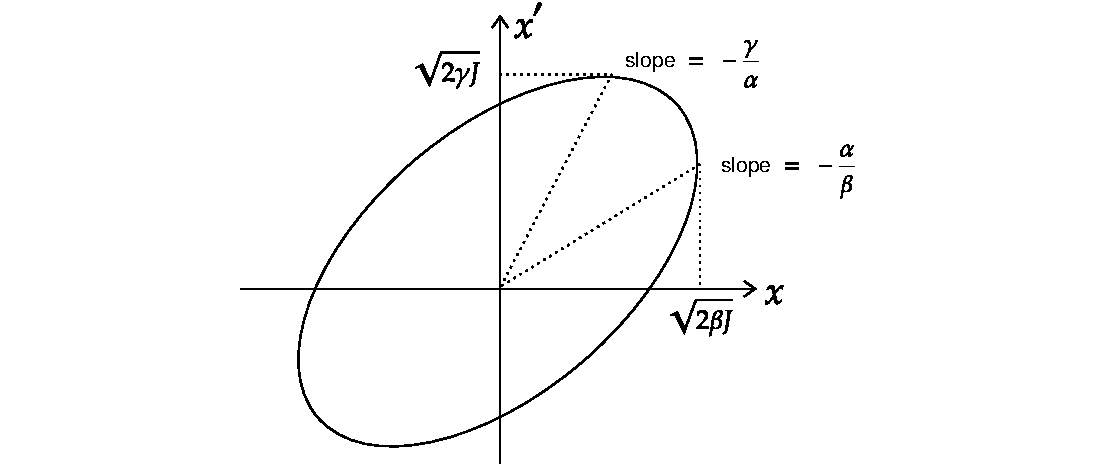
\includegraphics[width=0.5\textwidth]{Images/ellipse}
    \caption{Phase space ellipse traced by tur-by-turn (TbT) motion in the $(x,p_x)$ phase space. Optics functions determine the principal axes ratios and the inclination of the ellipse at each longitudinal position along the ring. From \cite{wolski_beam_2014}.}
    \label{ellipse}
\end{figure}
\section{Dispersive \& Chromatic Effecs and Linear Perturbations}
\subsubsection{Dispersion}
The equation of motion for off-momentum particles in the horizontal plane, the first of eqs.~\eqref{eq:linearEOM}, is a non-homogeneous Hill's equation. The solution consists on the linear combination of the homogeneous solution (betatron motion)  plus the particular solution: $x=x_\beta+ x_\delta$. Since the non-homogeneous term, $G(s)\delta$, is proportional to $\delta$, we can assume  $x_{\delta} = \eta(s)\delta$ where $\eta(s)$ is the \textit{dispersion function}, which should satisfy
    \begin{equation*}
        \eta^{\prime\prime}+(G^2+K)\eta=G,\quad
        \begin{cases}
            \eta(0) = \eta(L),\\
            \eta^\prime(0) = \eta^\prime(L).
        \end{cases}
    \end{equation*}
    The periodicity in the $\eta(s)$ function is required if we want to interpret it as a closed orbit distortion per relative momentum deviation. Thus, off-momentum particles perform betatron oscillations around a dispersive orbit, displaced from the nominal orbit by $\eta(s)\delta$. The dispersion function for the SIRIUS storage ring is shown in Fig.~\ref{dispersion_func}
    \begin{figure}[htb]
        \centering
        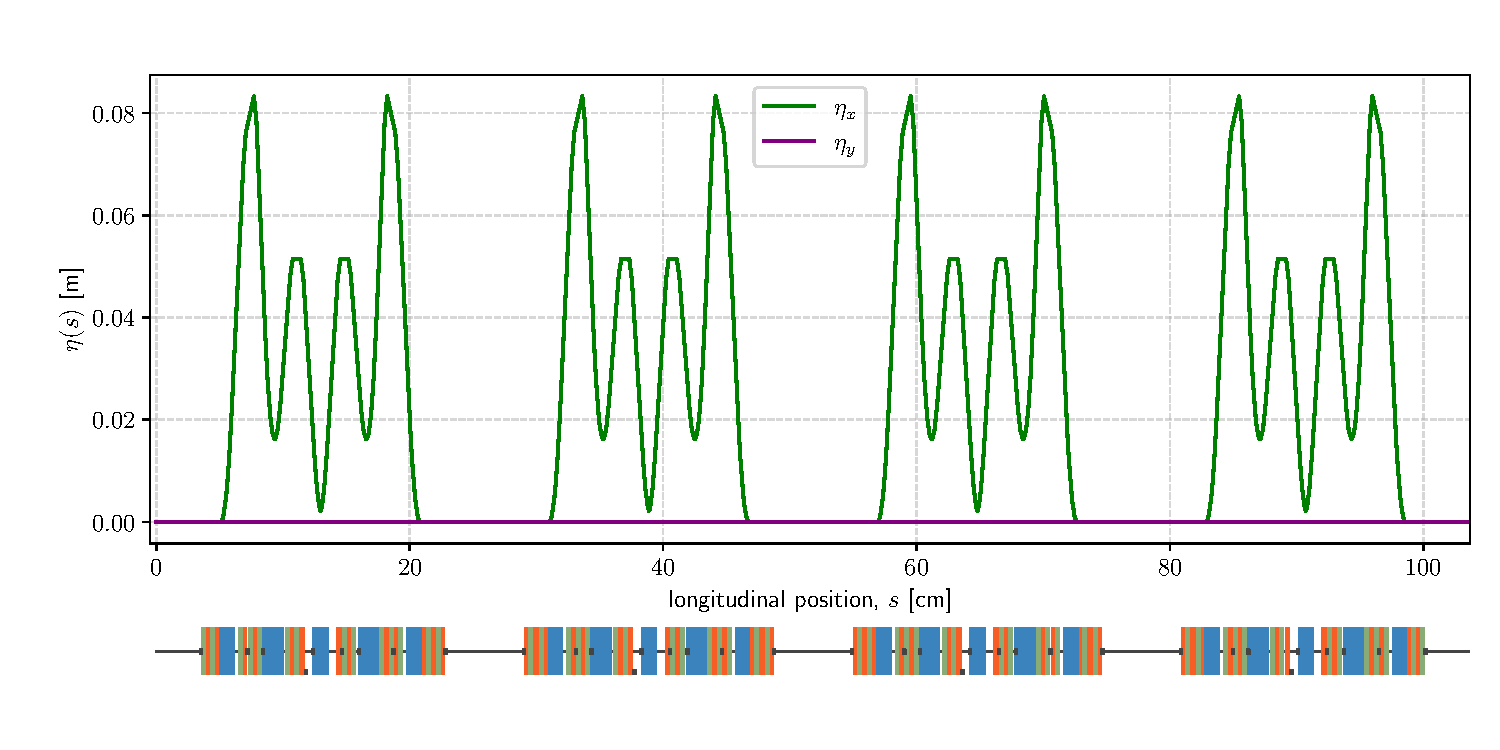
\includegraphics[width=\textwidth]{Images/dispersion.pdf}
        \caption{Dispersion fucntion for SIRIUS superperiod.}
        \label{dispersion_func}
    \end{figure}
    \subsubsection{Linear Field Errors}
    % The dipolar contributions promote additional bendgin and thud disturb the design orbit. Assuming the perturbations are not strong enough to kill the beam, a distorted closed orbit must exist. To find it we need to find the coordinates along the ring which are mapped to themselves after a complete revolution. That is, we must find the fixed point $\vb{X}_{\text{co}}$ of the disturbed one-turn map:
    % \begin{equation}
    %     \vb{X}_{\text{co}} = \mathbf{M} \vb{X}_{\text{co}} + \boldsymbol{\Delta}
    % \end{equation}
    % where $\boldsymbol{\Delta} = (0, \theta)^\intercal$, $\theta = B_y \Delta s / B\rho$ for the $(x, x^\prime)$ slice of the closed orbit, $\theta = B_x \Delta s / B\rho$ for the $(y, y^\prime)$. Solving for the closed orbit we find
    % \begin{equation}
    %     \vb{X}_{\text{co}} = (\mathbf{I} - \mathbf{M})^{-1}\boldsymbol{\Delta}.
    % \end{equation}
    % Using the Courant-Snyder parametrization for the one-turn map at the point $s_0$ immediately downstream the perturbation leads to
    % \begin{equation}
    %     \vb{X}_\text{co} = \frac{\theta}{2\sin\pi\nu}\mqty(\beta_0 \cos\pi\nu \\ \sin\pi\nu - \alpha_0 \cos\pi\nu).
    % \end{equation}

    In the presence of additional dipolar and quadrupolar fields representing field errors and deviations from the nominal fields, the orbit and focusing of the beam are changed. Assuming these are small perturbations and not sufficiently strong to kill the beam, we can evaluate the disturbances to the unperturbed dynamics. The details and derivations can be found in the literature, such as in chapter 2 of Ref. \cite{lee_accelerator_2004}. Here we highlight the main results.

    For dipole errors $\Delta G_y(s)=-\Delta B_{0x}(s)/R_0$ and $\Delta G_x(s)=\Delta B_{0y}(s)/R_0$, the equations of motion read
    \begin{equation}
        x^{\prime\prime}+K_x(s)x=G\delta + \Delta G_x(s), \quad
        y^{\prime\prime}+K_y(s)y = \Delta G_y(s).
        \label{eq:dip_errEOM}
    \end{equation}
    The solution consists on the combinations of the betatron motion plus the dispersive orbit (for the horizontal plane) plus the closed orbit distortion $u_{\text{co}}$ induced by the additional bending terms due to the dipole errors. For a single thin bending error $\Delta G_u$ in the $u=x,y$ plane, acting for a length $\Delta s$ around $s=s_0$, the closed orbit distortion $u_{\text{co}}$ reads
    \begin{equation}
        u_{\text{co}}(s) = \frac{\sqrt{\beta_u(s)\beta_u(s_0)}}{2\sin\pi\nu_u}\Delta G_u\cos( \pi\nu_u - |\phi_u(s)-\phi_u(s_0)|)\Delta s.
        \label{eq:cod}
    \end{equation}
    For a distribution $\Delta G_u(s)$ of dipolar perturbations along the ring, we sum over the contributions:
    \begin{equation}
        u_{\text{co}}(s) = \frac{\sqrt{\beta_u(s)}}{2\sin\pi\nu_u}\int_{s}^{s+L} \Delta G_u(\sigma)\sqrt{\beta_u(\sigma)}\cos(\pi\nu_u + \phi_u(s) - \phi_u(\sigma))\dd{\sigma}.
        \label{eq:co_dist}
    \end{equation}
    The prefactor involving the sine of the tune shows how $\nu_{u}$ close to an integer can amplify the effects of the dipolar perturbations on orbit distortions. At first sight, aiming for tunes half-integer tunes $\nu=k/2, k\in\mathbb{Z}$ might seem desireable to minimize the distortions. Choosing so, however, increases the sensitivity to gradient errors, which we examine next.
    % Knowledge of the beam-response to perturbations allows for the inversion of the problem. We can use specified small dipole kicks to correct the orbit, bringing it closer to the nominal one. These small dipole fields are generated by corrector magnets (CM's) abd orbit correction consists on linear problem of seeking CMs strength that minimze orbit distortions.

    % A quadrupole error can be represented by a thin-lens quadrupole transfer matrix \cite{Courant:1958wbj}
    % \begin{equation}
    %     \mathbf{M}_q = \mqty(1 & 0 \\ -k\Delta s & 1),
    %  \end{equation}
    %  so that, immediately downstream the error, the transfer matrix reads $\mathbf{M} = \mathbf{M}_q \mathbf{M}_0$. As a consequence, the optics deviates from the nominal optics. More notouriously, the beta and the phase advances, and thus tune, changes.

    %  The phase advance over a turn, $\phi$, is related to the trace of the one-turn transfer matrix $\mathbf{M}$ as $\cos\phi = 2 \tr \mathbf{M}$. Using the CS parametrization for $\mathbf{M}$, performing the multiplication $\mathbf{M}_q \mathbf{M}_0$ and calcualting the trace leads to
    %  \begin{equation}
    %     \cos \phi - \cos\phi_0 = - \frac{1}{2} k(s)\Delta s \beta_0 \sin\phi_0.
    %  \end{equation}
    %  In a linear approximation (if $\sin \phi_0$ is not near zero) $\Delta(\cos \phi) = \cos \phi - \cos\phi_0 \approx \Delta \phi\dv*{(\cos \phi)}{\phi}$ so the tune-shift due to a single thin-lens quadrupole error is

    Gradient errors can be modeled as corrections to the focusing functions in the equations of motion: $K_u(s)\to K_u(s) + \Delta K_u(s)$, for $\Delta K_x(s) = \Delta B_{1y}(s)/R_0$ and $\Delta K_y(s) = -\Delta B_{1x}(s)/R_0$. The changes in beam focusing lead to changes in the beta-functions, phase advances and consequently the betatron tunes. One can show the tune-shift as a consequence of a gradient error acting over a small extent $\Delta s$ around $s=s_0$ is \cite{lee_accelerator_2004}
         \begin{equation}
        \Delta \nu_u = \frac{1}{4\pi} \beta(s_0) \Delta K_u \Delta s.
        \label{eq:delta_nu}
     \end{equation}
     For a distribution of errors we sum over the ring:
     \begin{equation}
        \Delta \nu = \frac{1}{4\pi}\oint \beta(s) \Delta K(s) \dd s,
        \label{eq:delta_nu_dist}
    \end{equation}
    where the closed integration sign refers to a complete circulation along the ring, i.e., integration from $s_0$ to $s_0+L$, for any $s_0\in[0,L)$.

    %  Besides calculating the tune-shift, the resulting transfer-matrix for the lattice with errors allows for the identification of the new optics $\alpha, \beta, \gamma$, which can then be propagated to anywhere in the ring. In particular we can identify $\beta$ and its fractional deviation from the nominal value along $s$, a parameter known as \textit{beta-beating}
    As for the induced error on the beta-functions, it is possible to show that the relative error, known as betabeat, can be expressed as
     \begin{equation}
        \frac{\Delta \beta_u(s)}{\beta_u(s)} = - \frac{1}{2\sin(2\pi\nu_u)}\int_{s}^{s+L}\Delta K_u(\sigma)\cos[2(\phi_u(\sigma)-\phi_u(s)-\pi\nu)]\dd\sigma.
        \label{eq:beta_beat}
     \end{equation}
which is the largest for $2\nu_u$ closest to an integer. This means we must avoid tunes close to half-integers if we want to avoid the coherent build-up of betatron amplitudes, which can eventually lead to beam loss.
Integer or half-integer tunes are the simplest instances of resonances the beam can be subject to. A more general overview of resonances is presented in section 2.8.
\missingfigure{Int and HalfInt Ressonances Phase Space Diagrams}
\subsubsection{Chromaticity}
We know the bending angles at the dipoles is different for electrons with different energies. This is the origin of dispersive orbits. The energy deviations affect not only the closed orbit by means of the dispersion effect, but affect also the focusing of the trajectories, since a more/less energetic beam has higer/lower rigidity and thus is focused differently when passing through gradient fields.
%
% As for the higher order effect on the focusing, also known as chromatic effect, we consider the motion in a straight section under a gradient, so that there is no non-homogeneous term in the horizontal equation. The equation of motion considering $x\delta $ terms reads
% \begin{equation}
%     x^{\prime\prime}+(K_x+\Delta K_x)x=0
% \end{equation}
% \begin{equation}
%     y^{\prime\prime}+(K_y+\Delta K_y)y=0
% \end{equation}
% where $K_x=h^2+K_1$, e $K_y=-K_1$ and
Expanding the equations of motion, eqs.~\eqref{eq:EOMs}, for off-energy particles up to the order of terms $u\delta$, for $u=x,y$, reveals additional higher-order gradient errors. The focusing functions are corrected by $K_u(s)\to K_u(s) + \Delta K_u(s)$ \cite{lee_accelerator_2004,huang_beam-based_2019}, where
\begin{equation}
    \Delta K_x = -(K+2G^2)\delta \approx - K_x\delta
\end{equation}
\begin{equation}
    \Delta K_y = K\delta = - K_y\delta
\end{equation}
This means there exists an energy-dependent tune-shift effect caused by the gradient error. Using eq.~\eqref{eq:delta_nu_dist}, the tune-shift reads
% The result is that an off-momentum partcile sees a different optics along the ring: different beta function and different phase advance. Thus, it deviates from nominal operation conditions, specially in the tunes, inducing the tune-shifts
\begin{equation}
    \Delta \nu_u = - \frac{1}{4\pi}\oint\beta_u K_u \delta \dd{s},
    \label{eq:energy_delta_tune}
\end{equation}
for the $u=x,y$ planes. We can define the \textit{linear chromaticity} in the $u=x,y$ direction as tune-shift $\Delta \nu_u$ per relative energy deviation $\delta$:
\begin{equation}
    \xi_u=\dv{\nu_u}{\delta}.
\end{equation}
This uncorrected chromaticity is also called natural chromaticity. Using expression \eqref{eq:energy_delta_tune} for the tune-shift, the natural chromaticity reads
\begin{equation}
\xi_{u, \text {nat }} =-\frac{1}{4 \pi} \oint K_u \beta_u \dd{s}.
\end{equation}

This chromatic aberration effect needs to be corrected to guarantee energy-independent focusing. Correction can be attained with the insertion of geometric aberrations provided by sextupolar fields, specifically in the dispersive sections of the storage ring. In such regions, off-energy particles follow a dispersive orbit, and their position reads $x(s)=x_{\beta}(s)+\eta(s) \delta$, where $x_{\beta}(s)$ consists on the betatron oscillations. Since sextupolar fields are of the form
$$B_{x}=B_{2} x y, \quad B_{y}= \frac{B_{2}}{2}(x^{2}-y^{2}),$$
then, the off-momentum particles "see" the fields
$$B_{x}=B_{2}(x_\beta y + \eta \delta y), \quad B_{y}=\frac{B_{2}}{2}({x_\beta^{2}-y^{2}})+B_2 x_\beta \eta \delta + \frac{B_2}{2}(\eta \delta)^2,$$
So, to lowest order in eqs.~\eqref{eq:EOMs}, they feel a dipolar perturbation (which contributes to orbit distortions) and the gradient perturbation
$$\Delta K_{x,y}(\delta)=\pm S\eta \delta,$$
recalling that $S(s) = B_2 / R_0$.

Considering the contributions from both the errors induced by energy deviations and also the lowest order sextupole gradient effect, we have a total error of $\Delta K_u = -(K_u \mp S\eta)\delta$ to be inserted in eq.~\eqref{eq:delta_nu_dist}. The chromaticity in a lattice with sextupoles thus reads
\begin{equation*}
    \xi_{u}=-\frac{1}{4\pi}\oint\beta_{u}(K_{u}\mp S\eta)\dd s,
\end{equation*}
with the minus sign for $u=x$ and the plus sign for $u=y$. The chromaticity depends linearly on sextupole strengths, allowing for its correction to desired values. Since the effect of the sextupole field focuses in a given plane but defocuses in the other, at leas two sextupole families are requiered for chromaticity correction: one familiy where $\beta_x > \beta_y$ and other where $\beta_y < \beta_x$. The cost of correcting chromaticity is the insertion of perturbations and nonlinearities in the dynamics. To allow for more control over the nonlinear dynamics effects, usually some families of sextupoles are also placed in non-dispersive sections. They are called acrhomatic families, since they have no effect over chromaticity.
\missingfigure{show chromatic aberrations and their correction with geometric aberrations }

\section{Nonlinear Dynamics, Perturbations, Ressonances and Tune-Shifts}

\subsubsection{Action-Angle Variables}
Betatron motion of equation~\eqref{eq:Hill} can be obtained as Hamilton's equations for the effective, linear Hamiltonian
\begin{equation}
    \mathcal{H}=\frac{1}{2}u^{\prime2}+\frac{1}{2}K_u(s)u^2.
\end{equation}
A transformation $(u,u^\prime)\to(\psi, J)$ to Action-angle variables is implicitly implemented by the type-1 generating function
\begin{equation}
    F_1(u,\phi_u)=\int{u}^\prime\dd{{u}}=\frac{u^2}{2\beta_u}\qty(\tan \phi_u-\frac{\beta_u^\prime}{2}).
\end{equation}
The action variable reads
\begin{equation}
    J_u=-\pdv{F_1}{\phi_u} = \frac{u}{2\beta_u}\sec^2\phi_u = \frac{1}{2\beta_u}[u^2 + (\beta_u u^\prime + \alpha_u u^2)],
    \label{eq:action}
\end{equation}
from which we recover the pseudo-harmonic form $u=\sqrt{2\beta_u J_u}\cos(\phi_u(s)+\phi_0)$.

In the $J,\phi$ variables, the new hamiltonian is $H_0(\phi, J)$,  given by
\begin{equation}
    H_0=\mathcal{H}+\pdv{F_1}{s} = \frac{J}{\beta}.
\end{equation}
Performing the change to action-angle variable in both the horizontal and vertical planes we find the new Hamiltonian for 4D dynamics
\begin{equation}
    H_0= \frac{J_x}{\beta_x} +  \frac{J_y}{\beta_y},
\end{equation}
and Hamilton's equations read
\begin{equation}
    \phi_u^\prime = \frac{1}{\beta_u(s)},\qquad J_u^\prime=0.
\end{equation}
\subsubsection{Perturbations and tune-shifts}
Linear motion is integrable, since it can be written in terms of the action variable only (angle-independent Hamiltonian). This leads to the action variable being a constant of motion, and the phase advance behaving just as the pseudo-harmonic motion anticipated.

Linear motion, though, is only a useful first approximation. In reality, in an storage ring, there are higher order multipole magnets, such as sextupole magnets, and also multipole, alignement and excitation errors, all acting as perturbations to linear motion. Generically referring to perturbations as $V(J, \phi)$, we can write the perturbed motion Hamiltonian
\begin{equation}
    H(J,\phi) =H_0 + V(J,\phi).
\end{equation}
Hamilton's equations read
\begin{equation}
\phi_u^\prime = \frac{1}{\beta_u(s)}+\pdv{V(J,\phi)}{J_u}, \quad J_u^\prime = \pdv{V(J,\phi)}{\phi_u}.
\end{equation}
Since the tunes consist on the phase advance per revolution, we immediately see that the presence of perturbations leads to tune-shifts. Generically thus, the tunes can be expressed in terms of the tune-shifts as
$$\nu_0 = \nu_{u0} + \xi_u(\delta) \delta + \alpha_{uu} J_u + \alpha_{uv} J_v$$
where $\xi_u$ represents the energy-dependent tune-shifts (higher order generalization of linear chromaticity), and the other components consist on the amplitude-dependent tune-shifts, up to first order in the actions.


\subsubsection{Ressonances}
4D linear unperturbed motion consists on the motion of two uncoupled parametric oscillators. The phase-space is diffeomorphic to the 2-Torus, $\mathbb{T}^2$, and there are an infinite number of such tori, corresponding to the different choices of initial conditions $J_u$.

Canonical perturbation theory applied to perturbed motion fails to converge whenever the ratio of tunes is sufficiently rational. The Poincare-Birkhoff theorem states that under such conditions, almost all the periodic phase-space orbits disappear. An even number of tori survives, half of which are stable and half unstable. Unstable motion in a storage ring can eventually lead to beam loss.

The condition for sufficiently rational tunes can be expressed as
    $$m\nu_x + n\nu_y = \ell,$$
    for $n, m, \ell\in\mathbb{Z}$. This condition defines lines in tune-space corresponding to the locus in which perturbation theory fails and motion can become unstable. These are resonance lines and $|n|+|m|$ is the order of the resonance. Figure~\ref{resons} shows resonance lines for the resonances up to second, third and fourth order respectively. First order resonances can be excited by dipolar fields, 2nd order resonances can be excited by quadrupole fields and 3rd order resonances can be driven by sextupolar fields.
\begin{figure}[thb]
    \centering
    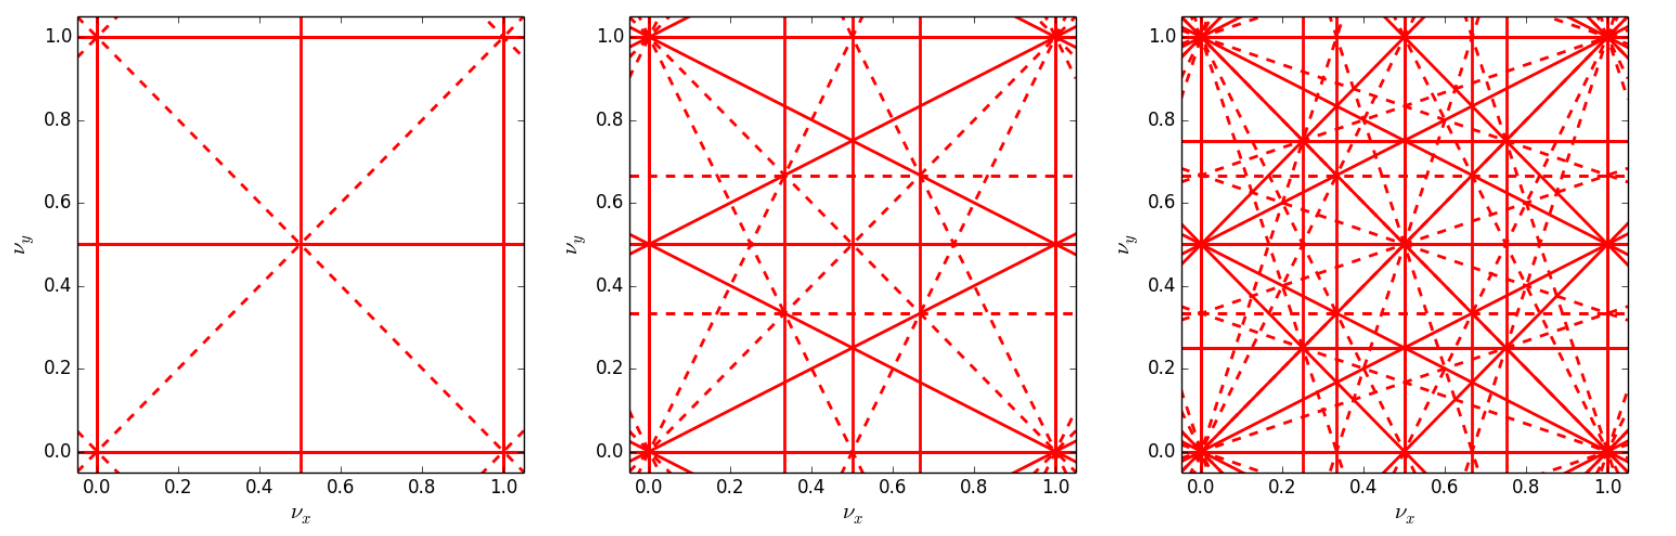
\includegraphics[width=\textwidth]{Images/tunes.png}
    \caption{Resonance lines in tune space up to 2nd, 3rd and 4th order, respectively.}
    \label{resons}
\end{figure}
\subsubsection{Dynamic Aperture}
    Nonlinear dynamics can become sensitive to initial conditions when the amplitudes are large. Because of the tune-shfits, specially the amplitude-dependent tune shifts, the tunes can wander in tune space, eventually crossing resonance conditions that may lead to instabilities, chatotic motion and beam loss. The dynamics can impose limitations to the maximum transverse deviations in which the beam can oscillate while displaying regular and bounded motion. This is a dynamic restriction to the motion known as the \textit{dynamic aperture}.

    Exceeding the dynamic aperture eventually leads to beam loss. During injection of the beam, if the transverse offsets are larger than the dynamic aperture, the beam is not captured into the storage ring. This is specially important for off-axis injection, such as in the case for SIRIUS.
